%----------------------------------------------------------------------------------------
%       PACKAGES AND THEMES
%
% docs: 
% https://en.wikibooks.org/wiki/LaTeX/Presentations#Introductory_example
% http://www.math-linux.com/latex-26/article/how-to-make-a-presentation-with-latex-introduction-to-beamer
%----------------------------------------------------------------------------------------


\documentclass{beamer}

\mode<presentation> {

% The Beamer class comes with a number of default slide themes
% which change the colors and layouts of slides. Below this is a list
% of all the themes, uncomment each in turn to see what they look like.

%\usetheme{default}
%\usetheme{AnnArbor}
%\usetheme{Antibes}
%\usetheme{Bergen}
%\usetheme{Berkeley}
%\usetheme{Berlin}
%\usetheme{Boadilla}
%\usetheme{CambridgeUS}
%\usetheme{Copenhagen}
%\usetheme{Darmstadt}
%\usetheme{Dresden}
%\usetheme{Frankfurt}
%\usetheme{Goettingen}
%\usetheme{Hannover}
%\usetheme{Ilmenau}
%\usetheme{JuanLesPins}
%\usetheme{Luebeck}
\usetheme{Madrid}
%\usetheme{Malmoe}
%\usetheme{Marburg}
%\usetheme{Montpellier}
%\usetheme{PaloAlto}
%\usetheme{Pittsburgh}
%\usetheme{Rochester}
%\usetheme{Singapore}
%\usetheme{Szeged}
%\usetheme{Warsaw}

% As well as themes, the Beamer class has a number of color themes
% for any slide theme. Uncomment each of these in turn to see how it
% changes the colors of your current slide theme.

%\usecolortheme{albatross}
%\usecolortheme{beaver}
%\usecolortheme{beetle}
\usecolortheme{crane}
%\usecolortheme{dolphin}
%\usecolortheme{dove}
%\usecolortheme{fly}
%\usecolortheme{lily}
%\usecolortheme{orchid}
%\usecolortheme{rose}
%\usecolortheme{seagull}
%\usecolortheme{seahorse}
%\usecolortheme{whale}
%\usecolortheme{wolverine}

%\setbeamertemplate{footline} % To remove the footer line in all slides uncomment this line
%\setbeamertemplate{footline}[page number] % To replace the footer line in all slides with a simple slide count uncomment this line

%\setbeamertemplate{navigation symbols}{} % To remove the navigation symbols from the bottom of all slides uncomment this line
}

%\usepackage[german]{babel}
\usepackage[latin1]{inputenc}
\usepackage{alltt}
\usepackage{beamerthemesplit}

\usepackage{graphicx} % Allows including images
\usepackage{booktabs} % Allows the use of \toprule, \midrule and \bottomrule in tables

\usepackage{color}
\usepackage{listings}
\lstset{
  %basicstyle=\ttfamily\bfseries,
  basicstyle=\ttfamily\footnotesize,
  commentstyle=\color{red}\itshape,
  stringstyle=\color{green},
  showstringspaces=false,
  keywordstyle=\color{blue}\bfseries,
  numberstyle=\ttfamily\tiny,
  frame=single,
  numbers=left,
  numbersep=1em,
  xleftmargin=2em,
  language=Python,
  breaklines=true,
  breakatwhitespace=true,
  postbreak=\hbox{$\hookrightarrow$ },
  showstringspaces=false,
  tabsize=2
}


%% pdf options
\hypersetup{pdfstartview={Fit}} % fits the presentation to the window when first displayed

%% Title Page

\title[Birdhouse]
{Birdhouse Web Processing Services}
\subtitle{A Use Case for the Climate Science Community}
\author{
Carsten Ehbrecht\\
\medskip
{\scriptsize \url{ehbrecht@dkrz.de}}
}
\institute{German Climate Computing Center (DKRZ)}
\date[April 2016]
{EGI Workshop: Design your e-Infrastructure\\
April 2016, Amsterdam}
\subject{Climate Science, Web Processing Service}




%------------------------------------------------

\begin{document}

%------------------------------------------------

  \begin{frame}[plain]
    \titlepage
  \end{frame}

%------------------------------------------------

\begin{frame}
\frametitle{Overview} % Table of contents slide, comment this block out to remove it
\tableofcontents % Throughout your presentation, if you choose to use \section{} and \subsection{} commands, these will automatically be printed on this slide as an overview of your presentation
\end{frame}

%------------------------------------------------

  \section{Use Case: Web Processing Service for Climate Data Processing}

%------------------------------------------------

  \begin{frame}[plain]
    \frametitle{Web Processing Service}
    A web service interface to standardize the way that algorithms are made available on the Internet.
    \begin{figure}
      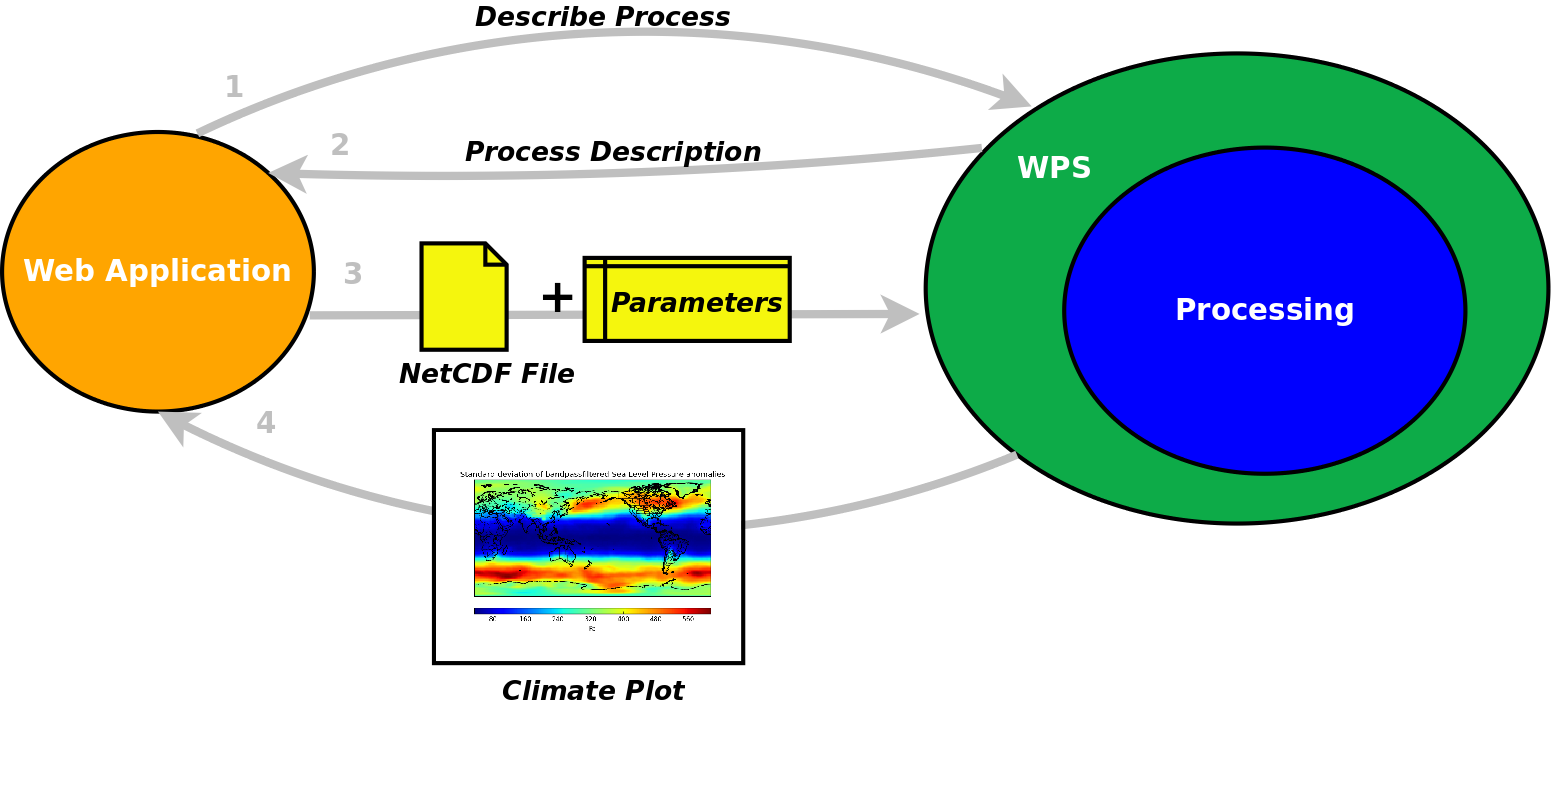
\includegraphics[width=12cm]{images/WpsUseCase.png}
    \end{figure}
    \setcounter{framenumber}{1}
    %\insertframenumber
  \end{frame}

%------------------------------------------------

  \begin{frame}[plain]
    \frametitle{Example: Ensemble Robustness Process}
    \begin{figure}
      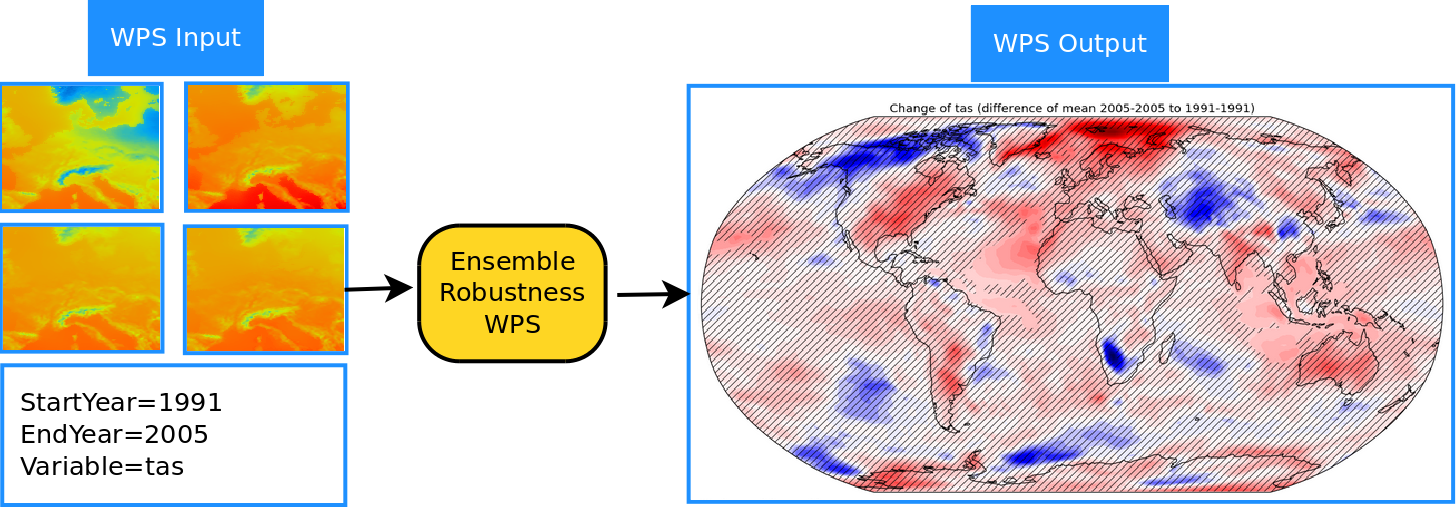
\includegraphics[width=12cm]{images/wps-ensemble-robustness.png}
    \end{figure}
    %\insertframenumber
   \end{frame}

%------------------------------------------------

  \begin{frame}[plain]
    \frametitle{Birdhouse WPS}
    \begin{figure}
      \includegraphics[width=4.5cm]{images/birdhouse-simple.png}
    \end{figure}
  \end{frame}


%------------------------------------------------

  \begin{frame}[plain]
    \frametitle{Birdhouse Overview}
    \begin{figure}
      \includegraphics[width=12cm]{images/birdhouse-components.png}
    \end{figure}
  \end{frame}

%------------------------------------------------

  \begin{frame}[plain]
    \frametitle{Using WPS in Copernicus}
    \begin{figure}
      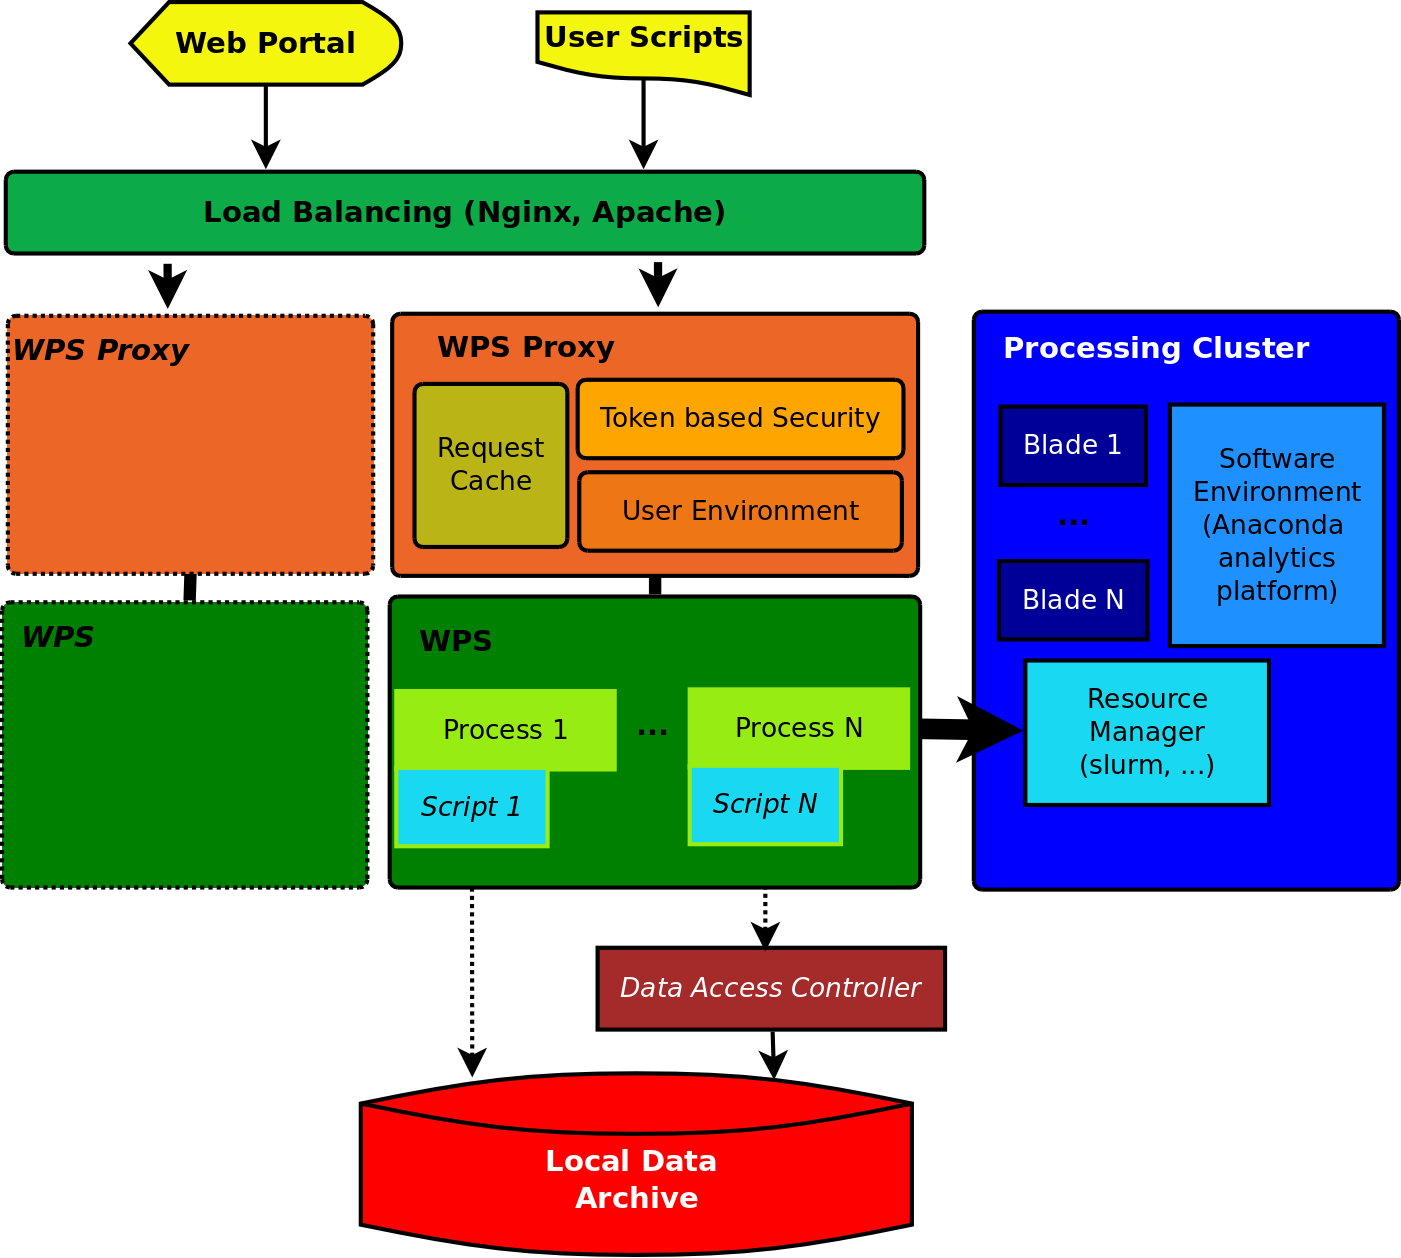
\includegraphics[width=9cm]{images/wps-copernicus-use-case.png}
    \end{figure}
  \end{frame}

%------------------------------------------------

  \begin{frame}[plain]
    \frametitle{Twitcher: WPS Security Proxy}
    \begin{figure}
      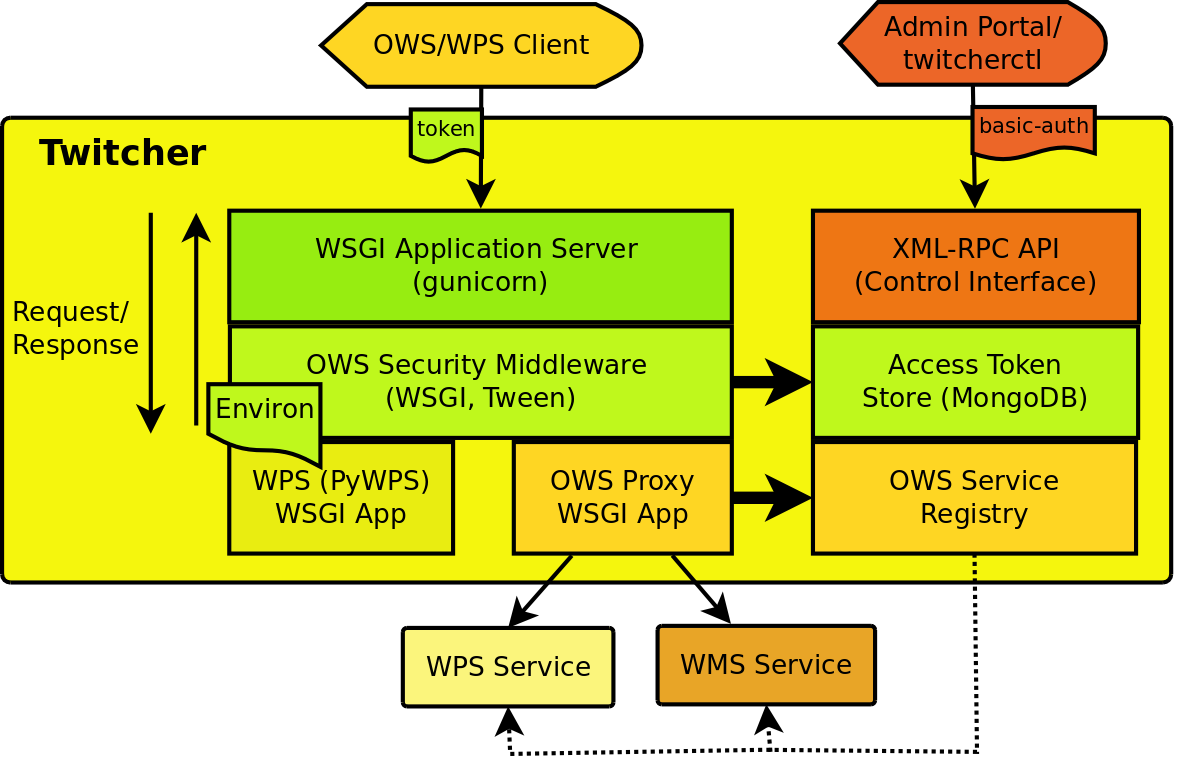
\includegraphics[width=12cm]{images/twitcher-overview.png}
    \end{figure}
  \end{frame}

%------------------------------------------------

  \section{Question and Answers}

  \begin{frame}[shrink]
    \frametitle{Background}
    \begin{block}{Who is the community the use case belongs to?}
      \begin{itemize}
        \item Climate data producers (metadata checks). 
        \item Users of climate data (impact modelers, forestry, biodiversity, ...).
        \item Decision makers (Copernicus).
      \end{itemize}
    \end{block}
    \begin{block}{What's the timeline for development, tests and large-scale operation?}
      \begin{itemize}
        \item Processing backend for Copernicus, starting in summer 2016, operational in 2019. 
        \item Climate metadata quality checks, development till summer 2016, operational end of 2016.
      \end{itemize}
    \end{block}
    \begin{block}{What's your role in the use case?}
      Providing the WPS infrastructure: deployment environment, security, test environment, attaching WPS to job schedulers like slurm, ... 
    \end{block}
  \end{frame}

%------------------------------------------------

   \begin{frame}[shrink]
    \frametitle{Users}
    \begin{block}{Who will be the users of the planned community-specific e-infrastructure? How many of them?}
      \begin{itemize}
        \item Scientists who work with or produce climate data (few to many).
        \item Decision makers (use a portal only, WPS is called via batch jobs).
      \end{itemize} 
    \end{block}
    \begin{block}{How will the users interact with the system?} % Show this on a system architecture diagram
      \begin{itemize}
        \item Most users will probably use a Web Portal which has access to the WPS services.
        \item Advanced users will use a command line and interact with the WPS services directly using scripts.
        %\item See next slide with the Copernicus Use Case.
      \end{itemize}
    \end{block}
    \begin{block}{Who and how would validate the system?}
      \begin{itemize}
        \item Scientists write algorithms which are published as WPS services.
        \item Functional tests provided by scientists to validate the results of the algorithms can be run in a continous integration environment (travis).
      \end{itemize}
    \end{block}
  \end{frame}

%------------------------------------------------

   \begin{frame}[shrink]
    \frametitle{Status}
    \begin{block}{Which components/services already exist in your architecture?}
      \begin{itemize}
         \item Deployment of WPS system (conda, buildout, docker). 
         \item Access to climate data sources (ESGF, Thredds, Cloud, ...).
         \item WPS clients (web based and terminal).
      \end{itemize}
    \end{block}
    \begin{block}{Which components/services are under development (and by who)?}
      \begin{itemize}
        \item Security proxy for WPS services (DKRZ, KNMI).
        \item Attaching job scheduler to WPS (DKRZ, BADC). 
       \end{itemize}
    \end{block}
    \begin{block}{Which components/services do you expect to get from EGI?}
      Usage of the EGI cloud resources?
    \end{block} 
  \end{frame}

%------------------------------------------------

   \begin{frame}[shrink]
    \frametitle{Plans for today}
    \begin{block}{What questions would you like to get answered today?}
      Is it possible to setup WPS on EGI cloud resources?
    \end{block}
    \begin{block}{What issues you would like to solve today?}
      Try an installation of a WPS service on EGI cloud.
    \end{block}
    \begin{block}{Other outcomes that you would like to get out from the workshop?}
      I'm new to EGI ... so just curious about the other Use Cases.
    \end{block}
  \end{frame}

%------------------------------------------------

  \appendix

  \section{Appendix}
  
   \begin{frame}[allowframebreaks]
    \frametitle<presentation>{Further Reading}    
    \begin{thebibliography}{10}    
      \beamertemplatearticlebibitems
    \bibitem{birdhouse}
      Birdhouse
      \newblock \url{http://bird-house.github.io/}
    \bibitem{c4i}
      Climate4Impact Portal
      \newblock \url{http://climate4impact.eu/impactportal/general/index.jsp}
    \bibitem{wps-cct}
      Web Processing Service
      \newblock \url{http://www.slideshare.net/GasperiJerome/20130530-web-processing-service-cct-cloud-toulouse-29423710}
   
    \end{thebibliography}
    
  \end{frame}
  
%------------------------------------------------

  \begin{frame}
    \Huge{\centerline{The End}}
  \end{frame}

%------------------------------------------------

\end{document}
